\documentclass[12pt,english]{scrartcl}

\usepackage{amsmath,amsfonts,amssymb,amscd,amsthm,amsbsy,alltt,bera,upref,fancyvrb}
\usepackage[T1]{fontenc}
\usepackage{babel}
\usepackage{graphicx}
\usepackage{tikz}

\textheight=10.0truein
\textwidth=6.5truein
\hoffset=-.5truein
\voffset=-.5truein
\pagestyle{headings}
\footskip=36pt
\swapnumbers
\DefineVerbatimEnvironment{code}{Verbatim}{fontsize=\small}
\DefineVerbatimEnvironment{example}{Verbatim}{fontsize=\small}

\usepackage{xcolor}
\definecolor{shade}{RGB}{240,255,255}
\definecolor{nw}{RGB}{255,239,213}

\makeatletter
    \setkomafont{section}{\color{white}%
        \bfseries\Large
        
\begin{tikzpicture}[overlay]
        \draw[fill=black] (0,-2pt) rectangle
        (\linewidth,16.4pt);
        \end{tikzpicture}}
    \setkomafont{subsection}{\color{black}%
        \bfseries\Large
        \begin{tikzpicture}[overlay]
        \draw[fill=white] (0,-2pt) rectangle
        (\linewidth,16.4pt);
        \end{tikzpicture}}

\def\and{%
  \end{tabular}%
  \hskip 1em \@plus.10fil\relax
  \begin{tabular}[t]{c}}
\makeatother
\makeindex

\title{Technical Report: The Austinites}
\author{
  Sheeyla Garcia\\
  \and
  Jesus Hernandez\\
  \and
  Kyle Nicola\\
  \and
  Stephen Ridings\\
  \and
  Carlos Rodriguez\\
  \and
  Mark Sandan\\  
}
\date{ August 7, 2014 }
\begin{document}
\thispagestyle{plain}
\maketitle
\tableofcontents

\begin{figure}[h!]
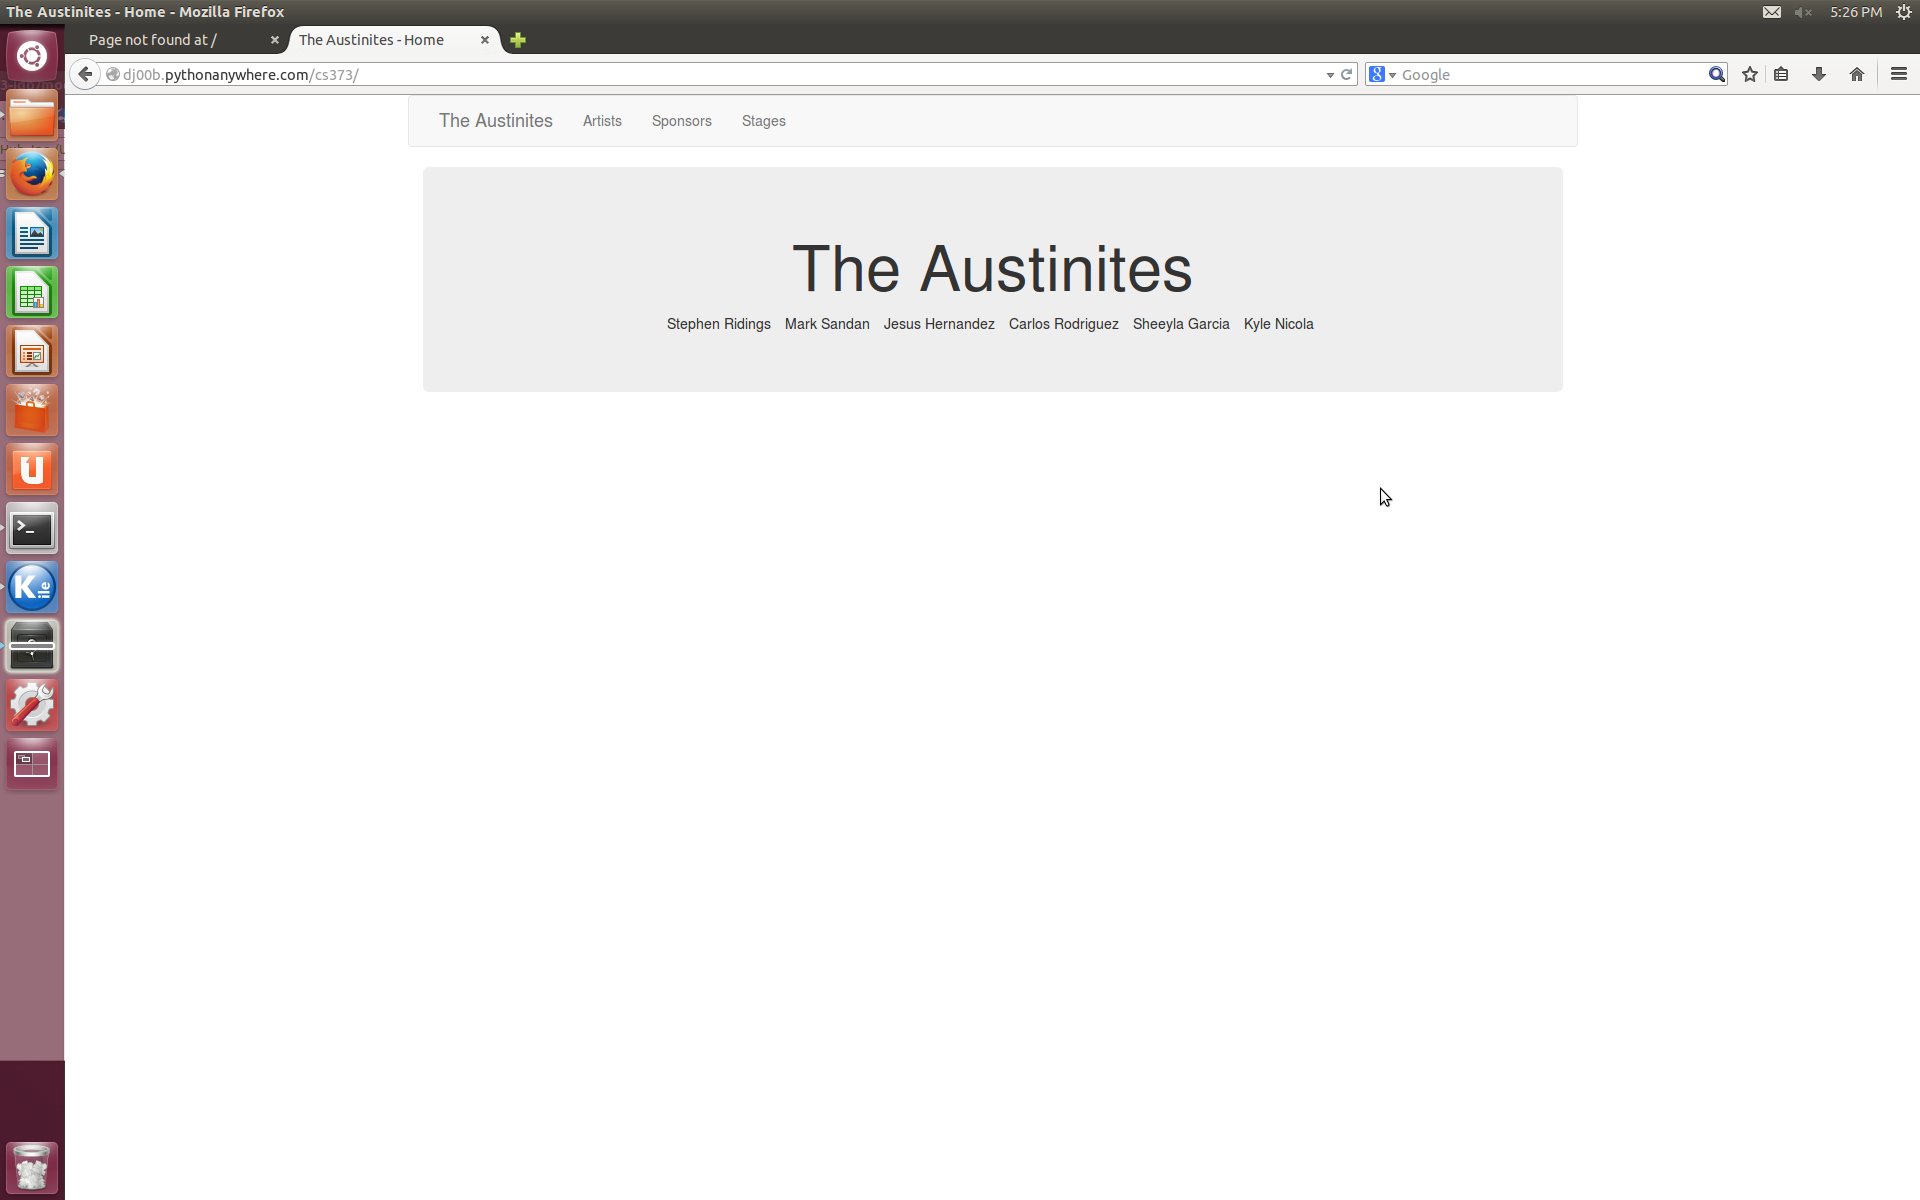
\includegraphics[width=\textwidth]{home.png}
 \caption{Splash Page for the second iteration of IDB2 showing the group name, buttons for the three main pages, and a link to the API on Apiary. The Carousel template from twitter bootstrap is used. 
          There is also a search bar added on the upper right.}
\end{figure}

\section{Updates}
Updates for the third iteration at a glance:
\begin{itemize}
 \item Search bar and Search Page listing result added
\end{itemize}
\begin{itemize}
 \item Augmented models to model time in relation to our models
\end{itemize}
\begin{itemize}
 \item Django Rest framework installed to implement the API and test it more rigorously including the new models
\end{itemize}
\begin{itemize}
 \item New API in apiary that includes information on the new classes to model time
\end{itemize}
\begin{itemize}
 \item New data added to the website that reflects the time relationships between models
\end{itemize}
\begin{itemize}
 \item New icons for the twitter, facebook, and youtube links along with an embedded google map on stages page
\end{itemize}
\subsection{Summary}
The main changes that have been made can be summarized into three categories: dynamic functionality, REST implementation, and the model refactoring. 

To implement a dynamic webpage we are currently using html,css,javascript, and the django template language to access instances of Artists, Sponsors, and Stages to fill the content of the webpages. 
The REST implementation required installing the django rest framework on the pythonanywhere envioronment which enabled us to return JSON representations of MySQL database instances. 
The tests for the REST implementation have also been added to the test suite.

The models have been refactored to include media classes that provide the dynamic content for the Artist,
Sponsor, and Stage models when they are loaded into the webpage. The media content contains embedded links to youtube, facebook, twitter, etc. 

Database loading has been relegated to using python scripts which have been installed as django commands used with manage.py. 
\section{Introduction}
Our website is about the 2014 Austin City Limits (ACL) music festival, an annual three-day American music festival that takes place on 46-acres in Zilker Park located in Austin, Texas. 
The website design has three main pages: Artists, Stages, and Sponsors along with a splash page. An Artist is allowed to perform on one stage but stages can have many artists perform on them.
A sponsor is a business entity that may or may not sponsor a stage. A stage is a physical location in the ACL festival that many artists play on. 
It can have only one sponsor that sponsors it for any given year. Artists and Sponsors are related through Stages.

The website allows anyone to view pages about the current Artists, Sponsors, and Stages involved in the festival. A user can find links from a specific artist page to the stage they're playing on
as well as the sponsor sponsoring the stage. Similarly for the stage and sponsor pages. The structure is modeled after the IMDB website (http://www.imdb.com/) where the entities are highly coupled.
A problem that we are facing is that the information we need to complete the project hasn't been published as of the date this report except the Artist lineup. Their scheduled performances which 
include information should be set to release sometime this month.

\section{New Features}
Our website is about the 2014 Austin City Limits (ACL) music festival, an annual three-day American music festival that takes place on 46-acres in Zilker Park located in Austin, Texas. 
The website design has three main pages: Artists, Stages, and Sponsors along with a splash page. An Artist is allowed to perform on one stage but stages can have many artists perform on them.
A sponsor is a business entity that may or may not sponsor a stage. A stage is a physical location in the ACL festival that many artists play on. 
It can have only one sponsor that sponsors it for any given year. Artists and Sponsors are related through Stages.

The website allows anyone to view pages about the current Artists, Sponsors, and Stages involved in the festival. A user can find links from a specific artist page to the stage they're playing on
as well as the sponsor sponsoring the stage. Similarly for the stage and sponsor pages. The structure is modeled after the IMDB website (http://www.imdb.com/) where the entities are highly coupled.
A problem that we are facing is that the information we need to complete the project hasn't been published as of the date this report except the Artist lineup. Their scheduled performances which 
include information should be set to release sometime this month.

\subsection{Search}
Currently our search functionality uses the Django haystack version 2.2.0 with the Whoosh python backend engine.
\subsection{New Models}




\subsection{Technology Stack}
The technologies used are:
\begin{itemize}
 \item PythonAnywhere: a web hosting service with python environments supported. Currently we use Python 3.4 and Django 1.6+.
\end{itemize}
\begin{itemize}
 \item Twitter Bootstrap 3.2: a web hosting service with python environments supported Python 3.4, Django 1.6.
\end{itemize}
\begin{itemize}
 \item Apiary: an online service to provide an API for client-side web access to our databases.
\end{itemize}
\begin{itemize}
 \item MySQL: The current database backend using the mysql.connector.django engine.
\end{itemize}
\begin{itemize}
 \item MySQL: The current database backend using the mysql.connector.django engine.
\end{itemize}
\section{Design}

Using Django's templating language we are able to reuse html files by extending from them. Currently we only have a single base html page that is extended from and 
uses Twitter Bootstrap. We have 24 pages that are dynamically loaded. The design and content of each page is outlined below.
\begin{figure}[h!]
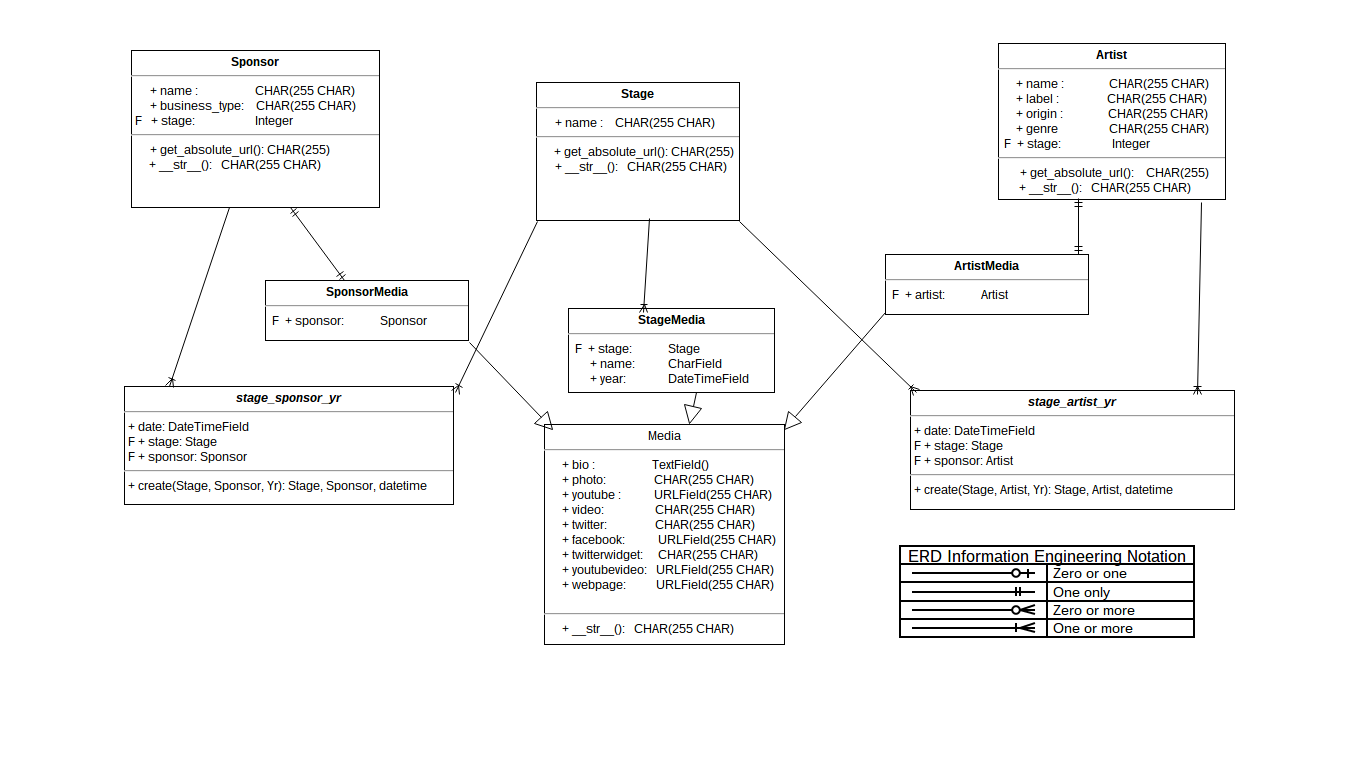
\includegraphics[width=\textwidth]{UML.png}
 \caption{The current UML schema depicting the relationships between the Django models. The main three models are Artist, Sponsor, and Stage each of which have an associated Media page.}
\end{figure}

\subsection{Web Pages}
Each web page has basic information about a particular artist, sponsor, or stage involved in the ACL music festival.
All pages will include  navigation links that will allow the user to go back to the main "splash" page, as well as reach the Artists, Sponsors, and
Stages pages. 

In future phases we are considering incorporating a search bar inside of the navigation bar, so that the user can search
all categories.

Mobile browsers are able to view the webpage correctly and set the height and width to a percentage of the size of the screen.
Using Django Templating along with Class-based Generic Views we were able to design a website that dynamically loaded pages using the information from our MySQL database.


\subsubsection{Splash Page}
\begin{itemize}
 \item URL: https://theaustinites.pythonanywhere.com/
\end{itemize}

The "splash" page will be the first page a visitor to the site will see. It provides button style links to all subcategories (Artists,
Sponsors, Stages). Currently the page uses the carousel template provided by twitter bootstrap.

\subsubsection{Artists}
\begin{figure}[h!]
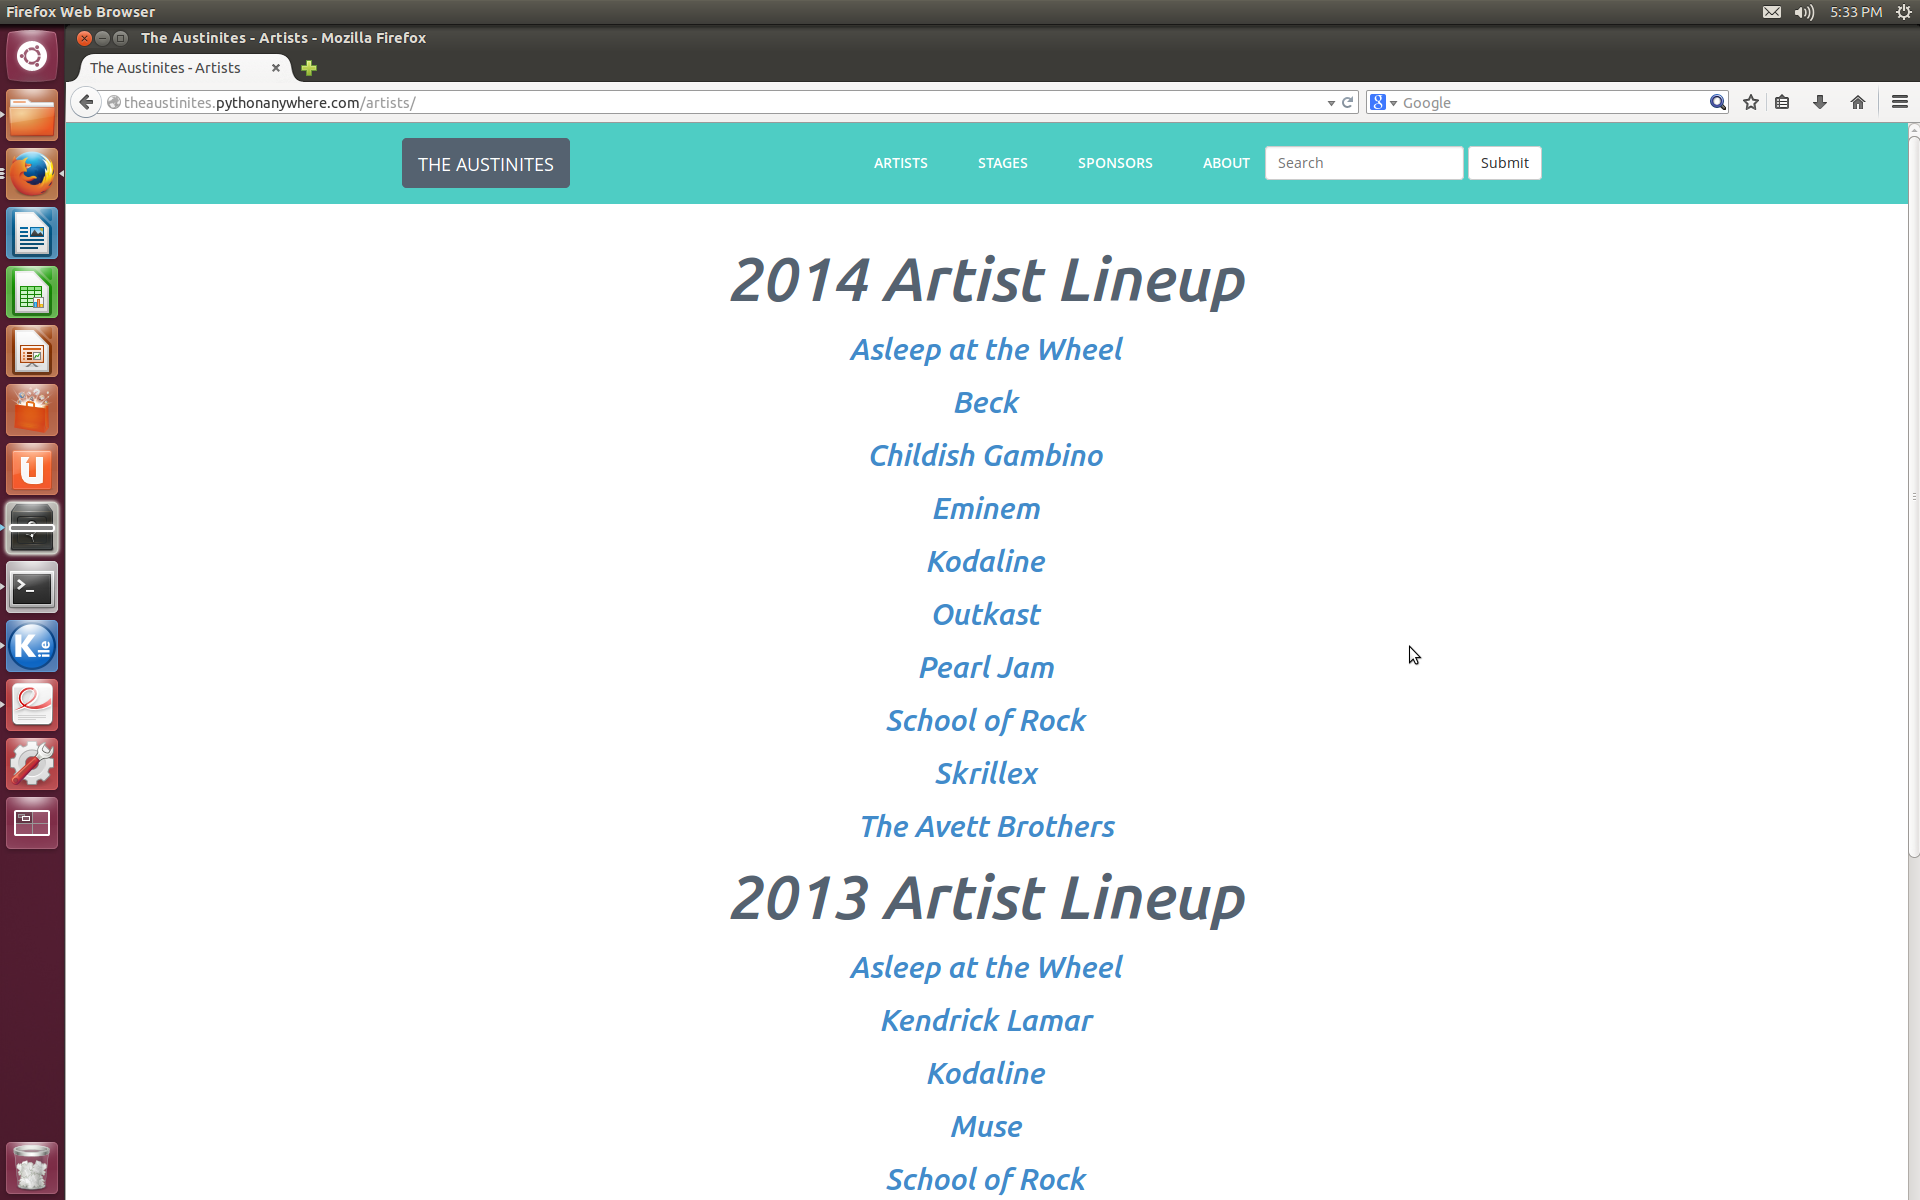
\includegraphics[width=\textwidth]{artists.png}
 \caption{The current UML schema depicting the relationships between the Django models. The main three models are Artist, Sponsor, and Stage each of which have an associated Media page.}
\end{figure}

\begin{itemize}
 \item URL: https://theaustinites.pythonanywhere.com/artists
\end{itemize}

Artist Pages can be reached from the home page as well as from the Stage or Sponsor pages depending on whether the Artist played on
a Stage that was hosted by a Sponsor.The page currently lists the dynamic web pages for music artists:
\begin{itemize}
 \item Outkast
 \item Eminem
 \item Pearl jam
 \item Beck
 \item Foster The People
 \item Skrillex
 \item Lana Del Rey
 \item Calvin Harris
 \item Phantogram
 \item Childish Gambino
\end{itemize}

Each Artist page includes the Artist name, an Artist photo, the label, the origin, genre, the sponsor,the stage, a bio,
the official website to the sponsor, a facebook page, a bio, youtube video, youtube channel, and twitter feed.

\subsubsection{Sponsors}
\begin{figure}[h!]
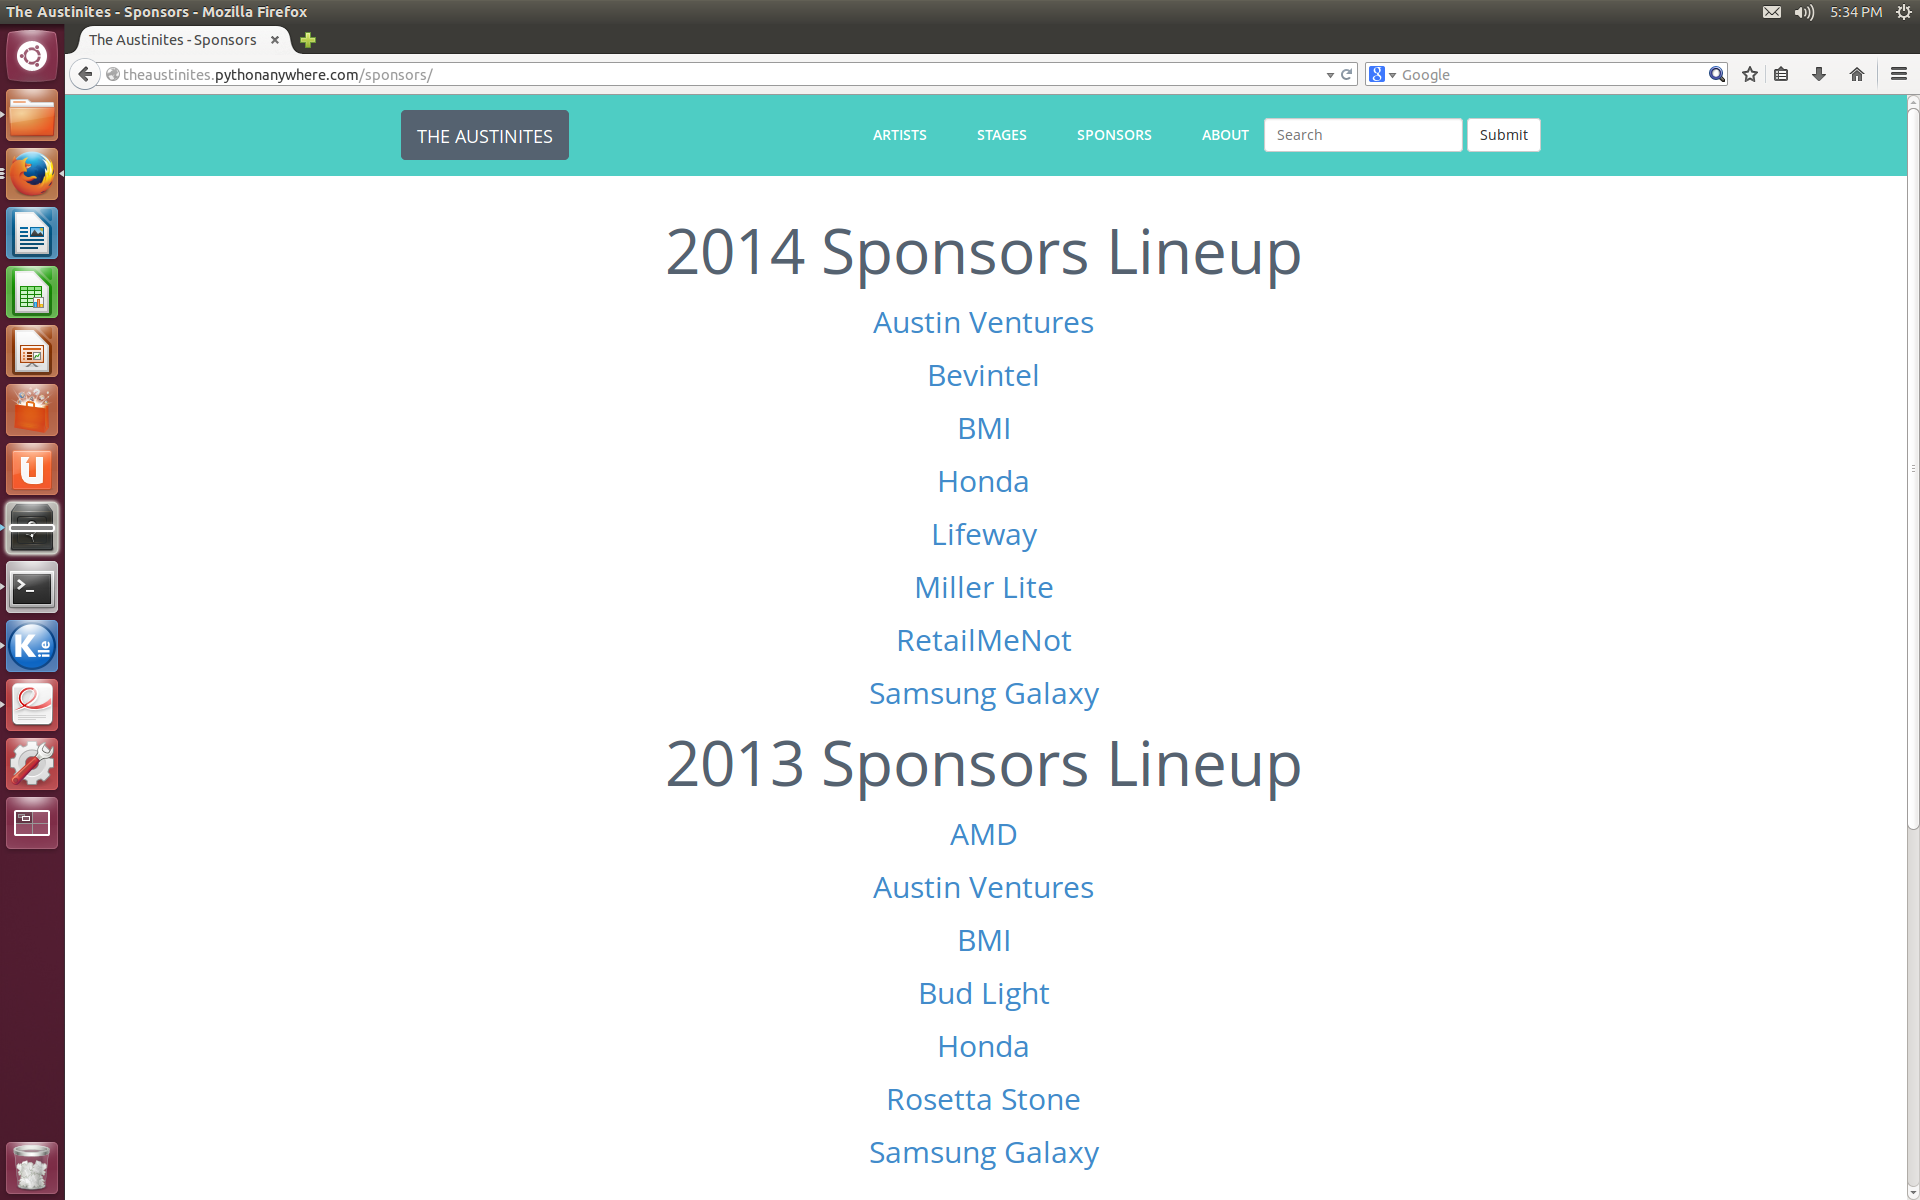
\includegraphics[width=\textwidth]{sponsors.png}
 \caption{The current UML schema depicting the relationships between the Django models. The main three models are Artist, Sponsor, and Stage each of which have an associated Media page.}
\end{figure}

\begin{itemize}
 \item URL: https://theaustinites.pythonanywhere.com/sponsors
\end{itemize}

Sponsor pages can be reached from the home page as well as from the Artist or Stages pages depending on whether the Sponsor hosted a
Stage, and that particular Artist played on that Stage. The page currently lists ACL festival sponsors:
\begin{itemize}
 \item Honda
 \item Miller Lite
 \item Samsung Galaxy
 \item Austin Ventures
 \item Bacardi
 \item BMI (Broadcast Music Inc.)
 \item Tito's Handmade Vodka
 \item H.E.B.
 \item Sweet Leaf Iced Teas
 \item Western Digital
\end{itemize}
Each Sponsor page includes the Sponsor name, a sponsor logo, the origin, stage sponsored, the artists playing the stage, the official website to the sponsor,
a facebook page, a bio, youtube video, and twitter feed.

\subsubsection{Stages}
\begin{figure}[h!]
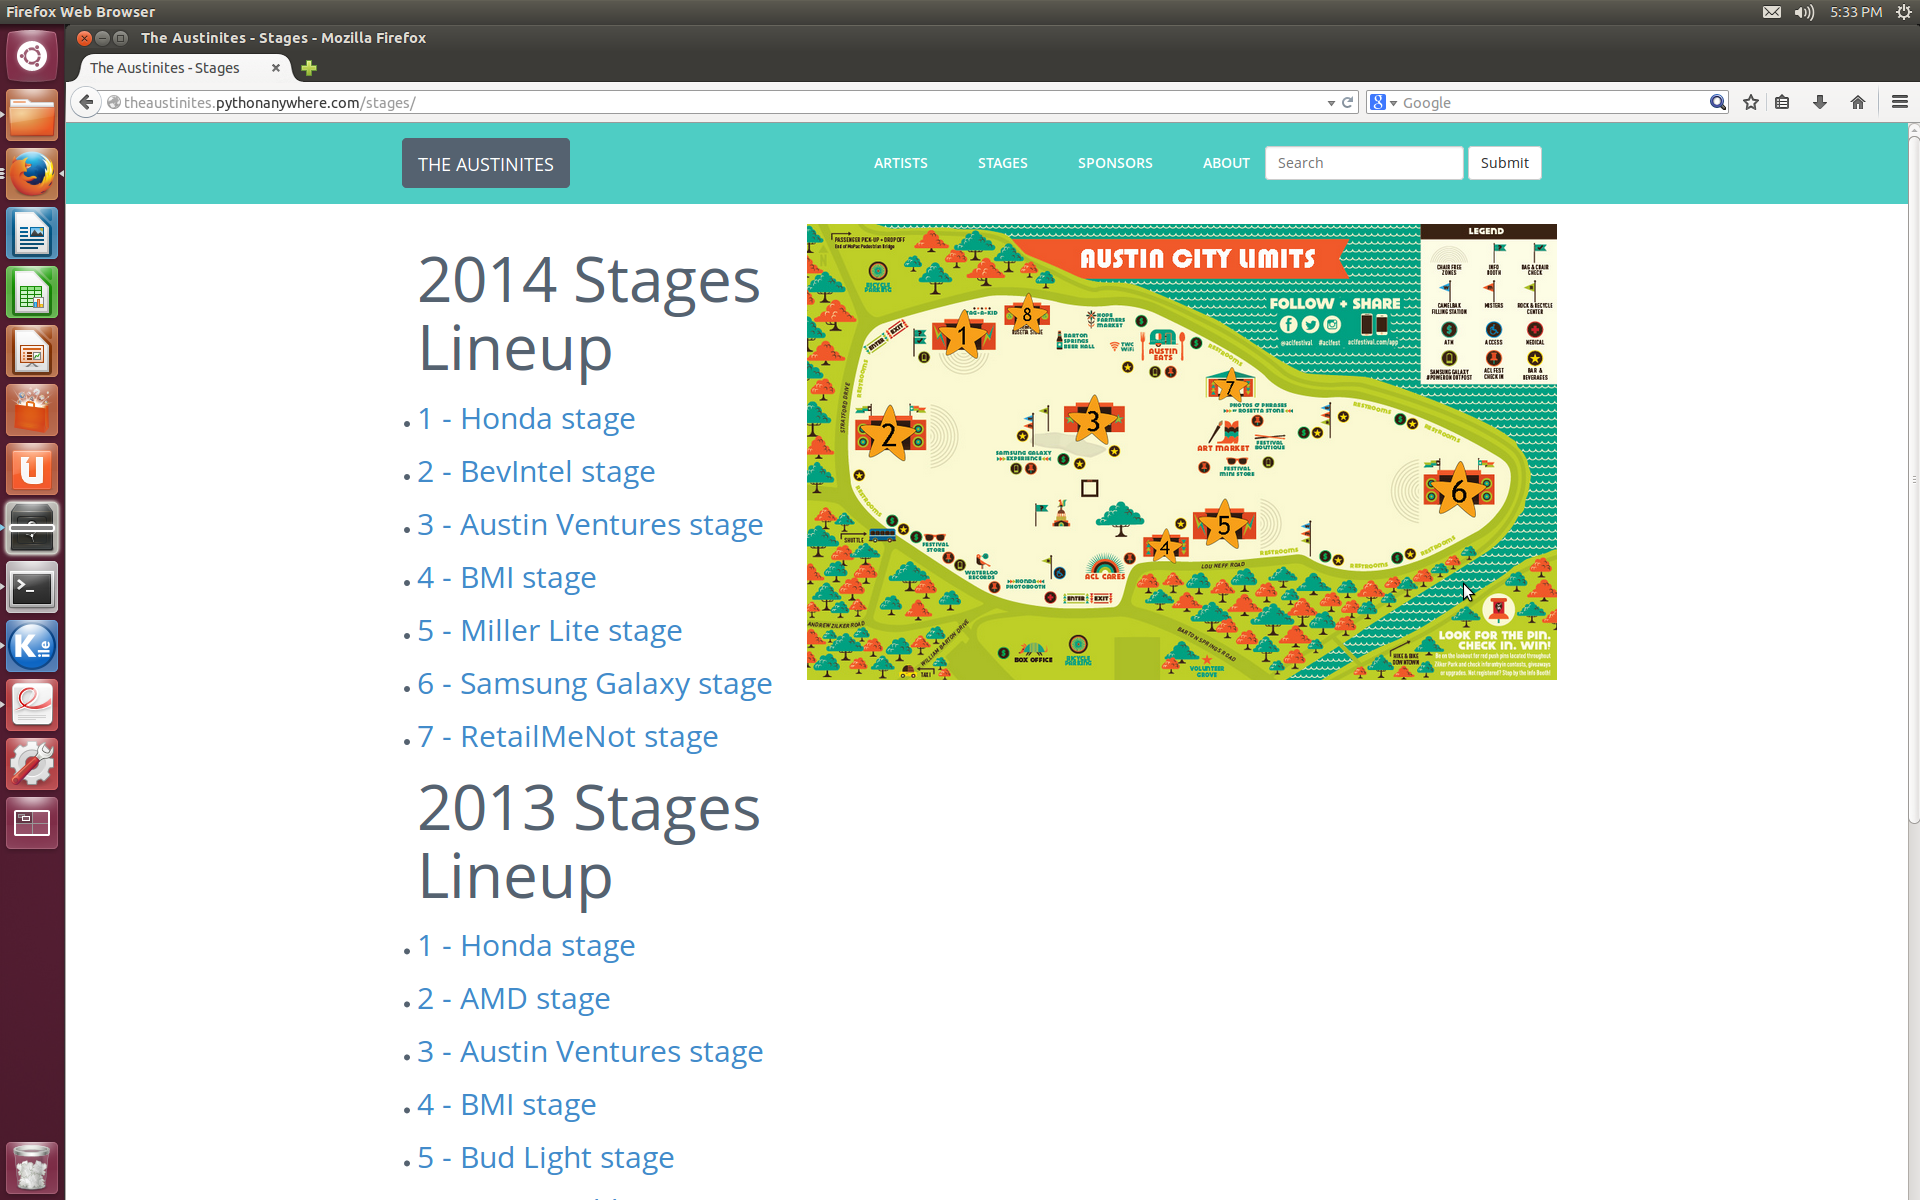
\includegraphics[width=\textwidth]{stages.png}
 \caption{The stages index page which features a map of the ACL festival at Zilker Park in Austin Texas. The numeric mapping is labeled here with stars.}
\end{figure}

\begin{itemize}
 \item Location: https://theaustinites.pythonanywhere.com/stages/
\end{itemize}

Stage pages can be reached from the Home page (splash) as well as from the Artist or Sponsor pages depending on whether the Sponsor hosted a
Stage, and that particular Artist played on that Stage. 

Each Stage page includes the Stage name, a Stage logo, the artists playing the stage, the official website to the sponsor,
a facebook page, youtube video, and twitter feed.

\subsection{Templates}
In phase one of the project we used Django templates to write static html files. In phase two we have updated our templates to use python code. Along with context from the views,
this allowed us to generate a dynamic website. Built-in methods from django models also allows us to access other related instances such as Stages and Sponsors for an Artist. We are able to 
provide links dynamically as new relationships are being added to the database.

\subsubsection{Base Template}
Our first template is base.html, which all other templates extend from. The template holds our bootstrap links as well as the main structure for the site.
We have separated the base template into sections labeled by the block keyword. Each template that extends base.html
can modify these sections to present a different site. This allows us to make new sites without rewriting code.

\subsubsection{Model Templates}
Each of the three main Models have their own templates. For example Artist has artists.html and artist.html. The plural template shows the list of artists using python to
iterate through the artist objects. The singular template uses python to access variables from the objects and call methods to display information.

\subsection{Class-based Generic Views}
We have rewritten our views for phase two of the project. Previously we used functions to render the html templates. We have moved to Class-Based Generic Views
that allow us to easily write views for common tasks. 

There are three main types of pages in terms of the 
generic view design: The splash page that uses the index function view, the Index pages that list
sponsors, artists, and stages, and the Detail pages that fill out content on a specific object's 
template.

\subsubsection{ArchiveIndexView}
The ArchiveIndexView generic class is used to pass the time relation objects which are automatically sorted 
by their date attribute. Using this class allowed us to easily pass the list of artists, stages, and sponsors to our templates.
Iterating through the list of objects we are able to dynamically load the page with the object's name and link to the other model classes they are related too.

\subsubsection{ListView}
The ListView generic class is used to pass the list of objects in the Model table into a template. We used this class in ArtistIndex, StageIndex, SponsorIndex.
Using this class allowed us to easily pass the list of artists, stages, and sponsors to our templates. Iterating through the list of objects we are able to dynamically
load the page with the object's name and link to the other model classes they are related too.

\subsubsection{DetailView}

The DetailView generic class is used to pass single objects from the database into a template. We used this
class in ArtistPage, StagePage, and SponsorPage. This class allowed us to pass an artist, sponsor, or stage to a template. Passing this information to the template allowed for the same template to represent different objects.

\subsection{RESTful  API}

The API allows GET requests to the following models: Stages, Sponsors, Artists. The  Members and Photos models have been deprecated since they haven't been used.
The following section will detail the attributes for the modules and how the server will respond to the GET requests. See 
the Links section below to view the Apiary API that outlines the GET responses for the Media models.

\subsubsection{Stages}

When a GET is called on $[/api/stages]$ it will return a JSON representation of all the Stages in the database.  It will be a list of the stages along with their attributes.
When a GET is called on $[/api/stages/{id}]$ it will return a JSON representation of a single Stage in the database with the given id.  It will list the stage and all of it's attributes
\\
Example of single stage:
\begin{verbatim}
{
         "location": 42,
}
\end{verbatim}
\subsubsection{Sponsor}

When a GET is called on $[/api/sponsors]$ it will return a JSON representation of all the Sponsors in the database.  It will be a list of the sponsors along with their attributes.
When a GET is called on $[/api/sponsors/{id}]$ it will return a JSON representation of a single Sponsor in the database with the given id.  It will list the sponsor and all of it's attributes.
\\
Example of single sponsor response:
\begin{verbatim}
{
        "id": 42,
        "name": "Sponsor name",
        "industry": "Type of Business",
}
\end{verbatim}

\subsubsection{Artist}

When a GET is called on $[/api/artists]$ it will return a JSON representation of all the Artists in the database.  It will be a list of the artists along with their attributes.
When a GET is called on $[/api/artists/{id}]$ it will return a JSON representation of a single Artist in the database with the given id.  It will list the artist and all of it's attributes.
\\
Example of single artist:
\begin{verbatim}
{
        "id": 42,
        "name": "Artist name",
        "label": "Label of artist",
        "origin": "Where the artist was from",
        "genre": "Genre of the artist",
        
}
\end{verbatim}



\subsection{Django Models}

The Django models created represent the entities we believe are essential to modeling the ACL festival.
The following subsections document the attributes and intended functionality of each class instance method. The following sections use
$child$ and $parent$ in the sense of the schema relationship depicted by the UML diagram in Figure 2 and not in the sense of the object oriented inheritance 
(the only object each model extends is models.Model except the Media classes ArtistMedia, SponsorMedia, and StageMedia that inherit from Media). Currently there are a total of six class.

\subsubsection{Artist}

The Artist class represents the current Artists playing on a sponsored stage. All Artists will be a child of some
stage depending on whether they are playing that Stage or not. The entity relation between Sponosor and Artist  The Artist class is implemented using the following:
\begin{verbatim}
attributes:
- id Primary Key, integer
- name: the unique name of max length 255 characters.
- label: the artist label with a maximum length of 255 characters.
- origin: the place of origin the artist/group formed with a 
          maximum length of 255 characters.
- genre: the genre associated with the artist. May span more 
         than one. maximum length of 255 characters.
- stage: Foreign Key, integer of type field.

methods:
- get_url(): returns the string "/artists/{id}" . Maximum number of 255 characters.
- __str__(): returns the name string of the artist.Maximum  number of 255 characters
\end{verbatim}


\subsubsection{Sponsor}

The Sponsor class represents the ACL sponsors that sponsor a Stage for the Artist to perform on.
This relationship is expressed using the one-to-many relationship between the Sponsor and the Stage
class. 

The Sponsor class has the following attributes and methods:
\begin{verbatim}
attributes:
- id: Primary Key, integer type field
- name: a character type field with a maximum length of 255 characters
- business_type: a character type field with a maximum length of 255 characters
- stage: Foreign Key, integer of type field

methods:
- get.url(): returns the string "/sponsors/{id}". Maximum number of 255 characters.
- __str__(): returns a string that represents the name of the sponsor.
\end{verbatim}

\subsubsection{Stage}

The Stage class is meant to represent the stage that an Artist will perform on. All stages
have one sponsor. The Stage class extends from the Django models.Models class.

The Stage class has the following attributes and methods:
\begin{verbatim}
attributes:
- id: Primary Key, integer type field
- name: a character type field with a maximum length of 255 characters


methods:
- get.url(): returns the string "/stages/%s/{name}" where name is the stage name.
- __str__(): returns a string that represents the name of the stage
\end{verbatim}

\subsubsection{stage\_sponsor\_yr}

The stage\_sponsor\_yr class is meant to relate a stage location with a sponsor in a given year.
The Stage class has the following attributes and methods:
\begin{verbatim}
attributes:
- id: Primary Key, integer type field
- date: a character type field with a maximum length of 255 characters
- stage
- sponsor

methods:
- get_absolute_url(): returns the string "/stages/%s/{name}" where name is the stage name.
- __str__(): returns a string that represents the name of the stage
\end{verbatim}

\subsubsection{stage\_artist\_yr}

The stage\_artist\_yr class is meant to relate a stage location with an artist in a given year.
The stage\_artist\_yr class has the following attributes and methods:
\begin{verbatim}
attributes:
- id: Primary Key, integer type field
- date: a character type field with a maximum length of 255 characters
- stage
- artist

methods:
- get_absolute_url(): returns the string "/stages/%s/{name}" where name is the stage name.
- __str__(): returns a string that represents the name of the stage
\end{verbatim}


\subsubsection{Media models}

The Media class will represent all of the media associated with Stages, Sponsors, and Artists. All Artists, Sponsors, and Stages will associated
with Media in a many-to-one relationship.

The Media class has been included to remove a lot of redundancy in code, and to simplify improving the overall 
design of our pages. We use the aggregation design pattern for each instance of a model and all Media classes will be an aggregate of all media
associated with an Artist, Stage, or Sponsor. The media components included will be images, videos, website,facebook,youtube channel and twitter feeds.

The Media class has the following attributes and methods
\begin{verbatim}
 attributes:
-id: Primary key, Integer
-bio: A CharField of 255 characters. Biography. 
-photo: A CharField of 255 characters. 
-youtube: A CharField of 255 characters. url for Youtube Channel
-video: A CharField of 255 characters.
-twitter: A CharField of 255 characters. url for Twitter
-facebook:A CharField of 255 characters. url for Facebook
-twitterwidget: A CharField of 255 characters.
-webpage: A Char field of 255 characters.
\end{verbatim}

\begin{verbatim}
methods:
- __str__(): returns a string that represent a stage, sponsor, or artist's website.

subclasses:
- SponsorMedia: a media subclass that has a one-to-one relationship 
                with an instance of the Sponsor class
  attributes:
  - sp: Foreign key, integer type field
- StageMedia: a media subclass that has a one-to-one relationship with 
              an instance of the Stage class
  attributes:
  - st: Foreign key, integer type field
- ArtistMedia: a media subclass that has a one-to-one relationship with an
               instance of the Artist class
  attributes:
  - ar: Foreign key, integer type field
  
\end{verbatim}

\subsubsection{Stage Sponsor Time relation}

The Media class will represent all of the media associated with Stages, Sponsors, and Artists. All Artists, Sponsors, and Stages will associated
with Media in a many-to-one relationship.

The Media class has been included to remove a lot of redundancy in code, and to simplify improving the overall 
design of our pages. We use the aggregation design pattern for each instance of a model and all Media classes will be an aggregate of all media
associated with an Artist, Stage, or Sponsor. The media components included will be images, videos, website,facebook,youtube channel and twitter feeds.

\subsubsection{Stage Artist Time relation}

The Media class will represent all of the media associated with Stages, Sponsors, and Artists. All Artists, Sponsors, and Stages will associated
with Media in a many-to-one relationship.

The Media class has been included to remove a lot of redundancy in code, and to simplify improving the overall 
design of our pages. We use the aggregation design pattern for each instance of a model and all Media classes will be an aggregate of all media
associated with an Artist, Stage, or Sponsor. The media components included will be images, videos, website,facebook,youtube channel and twitter feeds.

\section{Unit Tests}

The unit tests currently implemented reflect the expected functionality of the django models and database. they have been rigorously
augmented to test return values and simulations of corner cases. Currently we are using the MySQL database as a test database backend. 
We assume for each function in the set of tests that the state of the database is reset.There are currently 54 tests in the test suite testing the models and API.

\subsection{Django Model Unit Testing}
Currently the django models are tested with a MySQL database backend. The database created is temporary. It is created on setup, populated 
and run to test the attributes and methods of the models we use. Finally, when all tests are run the database is destroyed.
The tests are run in a non deterministic order. 

\subsubsection{Type Test}
Total tests: 3

\begin{itemize}
 \item test\_types: creates a Stage, Artist, and Sponsor and asserts their types ar Stage, Artist, and Sponsor respectively
 \item test\_types\_relationships1: tests different combinations of creating the stage_artist_yr object to relate a Stage and an Artist
 \item test\_types\_relationships2: tests different combinations of creating the stage_sponsort_yr object to relate a Stage and a Sponsor
\end{itemize}

\subsubsection{StageRelationship Test}
Total tests: 2

\begin{itemize}
 \item test\_relationship1: creates a Stage and an Artist and relates them with the stage_artist_yr object. Tests accessing the Stage and Artist from the stage_artist_yr.
 \item test\_relationship2: creates a Stage and a Sponsor and relates them with the stage_sponsor_yr object. Tests accessing the Stage and Sponsor from the stage_sponsor_yr.
 
\end{itemize}

\subsubsection{Constraint Test}
Total tests: 4
\begin{itemize}

\end{itemize} 

\subsubsection{MultiRelation Test} 
Total tests: 4

\begin{itemize}

\end{itemize}

\subsubsection{CrossRelation Test}

Total tests: 2

\begin{itemize}

\end{itemize}

\subsubsection{Simulations Test}

Total tests: 1

\begin{itemize}

\end{itemize}


\subsection{RESTful API Test} 

The REST API is tested using the django rest framework. The django rest framework has a built in library that allows the tests to mimic API clients that interact with the API.
Currently only GET requests are allowed. Any other request will return a 405 Method Not Allowed. There are three tests for each of the 
classes (Stages, Sponsors, Artists, ArtistMedia, StageMedia, and SponsorMedia). 

Each test sets up by creating mock relationships and attributes,
saving them to the database and then performing various GET requests using the client object from the django rest framework.

\subsubsection{Stages API Test} 
Total tests: 3
One stage with an id of 1 is uploaded into the database with name=$new stage$. On tear down, it is deleted.
\begin{itemize}
 \item testStageGet: tests the status code of a successful client requesting GET for the first stage.
 
 \item testStageGet2: tests the status code is 404 (Not Found) for an unsuccessful GET request for a stage instance
 that doesn't exist in the database.
 
 \item testPost: tests the status code is 405 (Method Not Allowed) for an unsuccessful POST request for the first stage.
\end{itemize}

\subsubsection{Artist API Test} 
Total tests: 3
A test stage and artist are uploaded into the database. On tear down they are both deleted.
\begin{itemize}
 \item testStageGet: tests the status code of a successful client requesting GET for the first artist
 
 \item testStageGet2: tests the status code is 404 (Not Found) for an unsuccessful GET request for an artist instance
 that doesn't exist in the database.
 
 \item testPost: tests the status code is 405 (Method Not Allowed) for an unsuccessful POST request for the first artist.
\end{itemize}

\subsubsection{Sponsors API Test} 
Total tests: 3
On setup one stage and one sponsor are created in the database and then deleted on tear down.
\begin{itemize}
 \item testStageGet: tests the status code of a successful client requesting GET for the first sponsor
 
 \item testStageGet2: tests the status code is 404 (Not Found) for an unsuccessful GET request for an sponsor instance
 that doesn't exist in the database.
 
 \item testPost: tests the status code is 405 (Method Not Allowed) for an unsuccessful POST request for the first sponsor.
\end{itemize}

\subsubsection{StageMedia API Test} 
Total tests: 3
On setup a stage and StageMedia are created in the database. Class attributes for the StageMedia test are created.
Both are deleted on tear down.
\begin{itemize}
 \item test\_stage\_media\_get: tests to see if a client request for the stage media object created returns the 200 OK response code.
 
 \item test\_stage\_media\_bad\_get: tests to see if a bad client request to a non-existing stage media object created returns 
                                     404 Not Found response.
 
 \item test\_stage\_media\_post: Tests that POSTS are not allowed by clients by checking that the 405 status code is returned.
\end{itemize}

\subsubsection{ArtistMedia API Test} 
Total tests: 3
On setup an artist, stage, and ArtistMedia are created in the database. Class attributes for the ArtistMedia test are created.
All instances are deleted on tear down.
\begin{itemize}
 \item test\_artist\_media\_get: tests to see if a client request for the artist media object created returns the 200 OK response code.
 
 \item test\_artist\_media\_bad\_get: tests to see if a bad client request to a non-existing stage artist object created returns 
                                     404 Not Found response.
 
 \item test\_artist\_media\_post: Tests that POSTS for artists are not allowed by clients by checking that the 405 status code is returned.
\end{itemize}

\subsubsection{SponsorMedia API Test} 
Total tests: 3
On setup a sponsor, stage, and SponsorMedia are created in the database. Class attributes for the SponsorMedia test are created.
All instances are deleted on tear down.
\begin{itemize}
  \item test\_sponsor\_media\_get: tests to see if a client request for the sponsor media object created returns the 200 OK response code.
 
 \item test\_sponsor\_media\_bad\_get: tests to see if a bad client request to a non-existing sponsor media object created returns 
                                     404 Not Found response.
 
 \item test\_sponsor\_media\_post: Tests that POSTS for sponsors are not allowed by clients by checking that the 405 status code is returned.
\end{itemize}


\section{Six Potters API Testing}


\section{Links}

\begin{itemize}
 \item Home Page: https://theaustinites.pythonanywhere.com/
 \item Apiary API: http://docs.aclapi.apiary.io/
 \item Github: https://github.com/sandan/cs373-idb
 \item http://www.aclfestival.com/
\end{itemize}

\end{document}